\documentclass[border=10pt]{standalone}
\usepackage{pgfplots}
\pgfplotsset{compat=1.18}
\usepgfplotslibrary{fillbetween}
\begin{document}
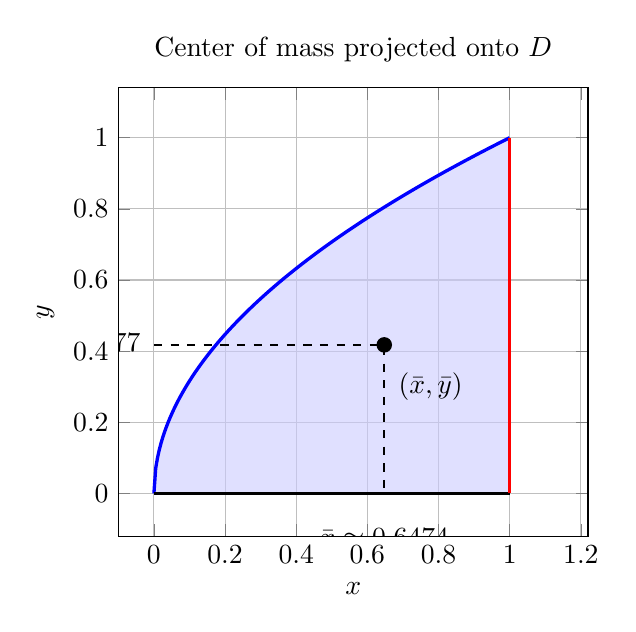
\begin{tikzpicture}
\begin{axis}[
    axis equal image,
    xmin=-0.10,xmax=1.22,ymin=-0.12,ymax=1.14,
    xlabel={$x$}, ylabel={$y$},
    title={Center of mass projected onto $D$},
    grid=both,
    samples=200,
]
\addplot[name path=A, domain=0:1, blue, very thick] {sqrt(x)};
\addplot[name path=B, domain=0:1, black, thick] {0};
\addplot[blue!20, opacity=0.6] fill between[of=A and B];
\addplot[red, very thick] coordinates {(1,0) (1,1)};
\draw[dashed, thick] (axis cs:0,0.4177) -- (axis cs:0.6474,0.4177) -- (axis cs:0.6474,0);
\addplot[only marks, mark=*, mark size=2.6pt, black] coordinates {(0.6474,0.4177)};
\node[right] at (axis cs:0.66,0.30) {$(\bar x,\bar y)$};
\node[below] at (axis cs:0.6474,-0.07) {$\bar x\approx0.6474$};
\node[left] at (axis cs:-0.01,0.4177) {$\bar y\approx0.4177$};
\end{axis}
\end{tikzpicture}
\end{document}
